\documentclass[letterpaper, 10 pt, conference]{ieeeconf}
\IEEEoverridecommandlockouts
\overrideIEEEmargins

\usepackage{cite}
\def\citepunct{,}
\def\citedash{--}
\usepackage{graphicx}
\usepackage{booktabs}
\usepackage{amsmath,amsfonts}
\usepackage{multirow}
\usepackage[bookmarks=true]{hyperref}
\hypersetup{breaklinks, colorlinks=true, linkcolor=black, urlcolor=black, citecolor=black}
\usepackage{algorithm}
\usepackage[noend]{algpseudocode}

\begin{document}
\bstctlcite{IEEEexample:BSTcontrol}

\title{\LARGE \bf Risk-Aware Active Perception and Planning \\ for Crowd Navigation Under Limited Sensing}

% TODO: confirm the affiliations
\author{James Zhu$^{1}$, Ahmed Ahmed$^{1}$, William Chan Santos$^{2}$, Pinhas Ben-Tzvi$^{1}$%
\thanks{$^{1}$Department of Electrical and Computer Engineering, University of Miami, Coral Gables, FL, USA}%
\thanks{$^{2}$Department of Biomedical Engineering, University of Miami, Coral Gables, FL, USA}%
}

\maketitle
\thispagestyle{empty}
\pagestyle{empty}

\section{Preliminaries and Definitions}

\textit{a) The problem:} A robot navigating a crowd with one onboard camera sees a 60$^\circ$ cone to a range of 4\,m in front of it. Pedestrians outside the cone are invisible, so people crossing in from the side are detected late and the tracks of people who leave the view grow stale. We give the camera a pan joint and ask the planner to decide where it looks. The question of this project is what objective should drive that decision, and how much it buys. The robot is a unicycle with state $(x, y, \theta, \phi)$, $\phi$ the pan angle, and inputs $(v, \omega, \omega_\phi)$; it plans at 2.5\,Hz over a horizon of $N{=}8$ steps of 0.4\,s. Pedestrians are replayed from the ETH/UCY recordings and do not react to the robot.

\textit{b) Modules:} Every 0.4\,s the camera returns detections, a tracker turns them into a belief over all pedestrians, a predictor turns each track into a Gaussian trajectory, and the planner solves one optimization for the motion and the camera. The four modules (Fig.~\ref{fig:socnav}) are the ones described below; all gaze strategies we compare share the first three and differ only in the planner's camera term.

\textit{c) Chance-constrained MPC:} The planner is SupeR-MPC~\cite{zhu2025robust}, a robust MPC whose constraints are tightened by the propagated uncertainty of the robot's own state, parameters and process noise. For a tracked pedestrian $j$ with predicted position $\mu_{jk}$ and covariance $\Sigma_{jk}$ at step $k$, the collision constraint is a half-plane with a back-off,
\begin{equation}
a_{jk}^\top(c_{r,k}-\mu_{jk}) - r_\text{c} \ge \kappa_j \sqrt{2\,a_{jk}^\top(\Sigma_{r,k}+\Sigma_{jk})\,a_{jk}},
\label{eq:cc}
\end{equation}
where $a_{jk}$ is the direction from the pedestrian to the robot, $r_\text{c}$ the sum of the two radii, $\Sigma_{r,k}$ the robot's position covariance, and $\kappa_j=\operatorname{erf}^{-1}(1-2\min(\delta/r_j,\tfrac12))$ sets the risk $\delta{=}0.05$. The existence probability $r_j$ of the track enters through $\kappa_j$: a track that may be a ghost is constrained less. The right-hand side is the \emph{back-off}: the distance the robot keeps beyond contact because it is unsure where the pedestrian will be. Everything the camera can do for the planner it does through this term.

\textit{d) The Poisson multi-Bernoulli tracker:} A Kalman tracker knows only the people it has seen. A PMB tracker~\cite{williams2015marginal} adds a model of the people it has not. It keeps two things. \emph{Bernoulli tracks} for detected pedestrians, each with an existence probability $r_j$ and a Gaussian constant-velocity state. A detection sets $r_j{=}1$; a step in which the camera looked where the track should be and saw nothing lowers it, $r_j \leftarrow r_j(1-p_D)/(1-r_j p_D)$; a step in which the track was out of view leaves $r_j$ alone and lets the covariance grow. Tracks are dropped once their position standard deviation exceeds 1\,m, since a stale track that blocks half the corridor is worse than none. The second object is a \emph{Poisson intensity} $D$ of undetected pedestrians on a 0.25\,m grid with five direction channels: $D$ summed over a region is the expected number of people there whom the robot has never seen. It starts as the scene's mean occupancy, fitted on the first half of each recording as a map of where people walk; each step it is advected along the learned flows, diffused, and multiplied by $1-p_D$ in every cell the camera could see (Fig.~\ref{fig:ppp}). Looking somewhere and seeing nobody therefore \emph{empties} that part of the map, which is the mechanism that lets a camera reduce the risk from people it has not detected. A scene-wide multiplier $\lambda \sim \mathrm{Gamma}(a, b)$ rescales $D$ online when more people appear than the prior expects; it makes the number of undetected pedestrians in a region $A$ negative binomial, with $P(\text{none in } A) = (b/(b+D(A)))^a$.

\begin{figure*}[t]
\centering
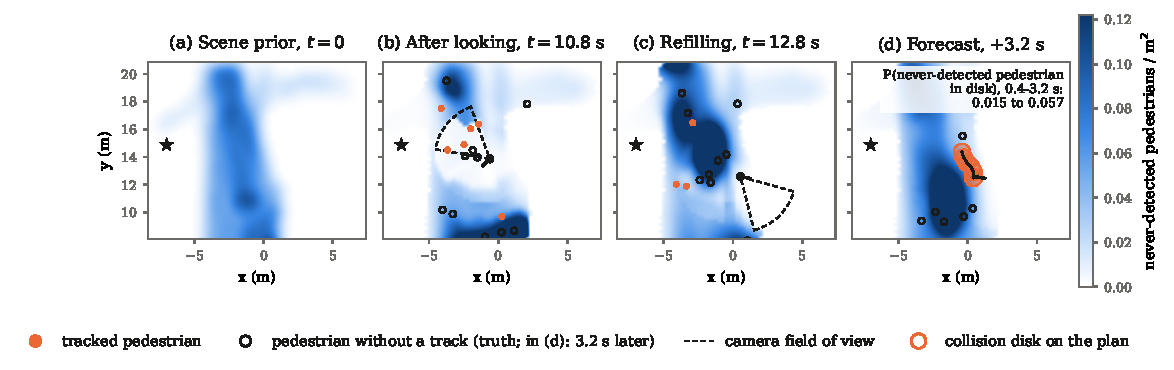
\includegraphics[width=0.96\textwidth]{fig_ppp.pdf}
\caption{The Poisson part of the tracker in one Zara episode. (a) The prior intensity of never-detected pedestrians. (b) Looking clears the intensity inside the camera's view (dashed). (c) Cleared areas refill as people walk in, and pruned tracks return to the intensity. (d) The intensity predicted 3.2\,s ahead without measurements, and the probability of a never-detected pedestrian in each collision disk on the planned path, which the unseen-pedestrian constraint bounds. Hollow circles: pedestrians without a track (ground truth; in (d) their positions 3.2\,s later). Dots: tracked pedestrians.}
\label{fig:ppp}
\end{figure*}

\textit{e) Prediction:} Each track's history feeds a Social LSTM~\cite{alahi2016social} that outputs a Gaussian position for every horizon step. The network is trained leave-one-scene-out, so the scene being evaluated is never in its training data, with random rotations of the training trajectories: without them the predictor was twice as bad on ETH, whose crowd walks along the other axis. The predicted covariance is the sum of the network's spread and the track covariance propagated with constant velocity; it is what \eqref{eq:cc} uses, and it is calibrated: 96\% of true positions fall inside the 95\% ellipse.

\textit{f) Unseen pedestrians in the planner:} The intensity gives a second chance constraint per step: the forecast undetected mass inside the robot's collision disk must stay below the mass $M(\delta_u)$ at which $P(\ge 1 \text{ undetected pedestrian}) = \delta_u{=}0.02$. It uses the intensity as it is now, propagated without future measurements, so safety never relies on a view not yet taken.

\textit{g) Risk-aware gaze:} The camera cannot change the constraints, which use current information, but it can change what the constraints will look like at the next replans. The cost therefore rewards camera motions that shrink the \emph{expected} back-off. With a smooth visibility $\mathrm{vis}_{jk}$ (field of view times range) of pedestrian $j$ from the planned pose at step $k$, and $\pi_{jm}$ the probability it is first seen at step $m$, the expected covariance after the planned views is
\begin{equation}
\begin{aligned}
\tilde\Sigma_{jk} = \Sigma^\text{model}_{jk} &+ \textstyle\prod_{m\le k}(1-\mathrm{vis}_{jm})\,\Sigma^\text{state}_{jk}\\
&+ \textstyle\sum_{m\le k}\pi_{jm} J_{k-m}P_\infty J_{k-m}^\top,
\end{aligned}
\label{eq:exp}
\end{equation}
where the reducible part $\Sigma^\text{state}$ survives only if no view catches the pedestrian, and a first sighting at $m$ resets it to the steady-state track covariance $P_\infty$ propagated $k-m$ steps. The cost adds $w\,\rho_{jk}\,\kappa\sqrt{2a_{jk}^\top(\Sigma_{r,k}+\tilde\Sigma_{jk})a_{jk}}$ for the most collision-relevant pedestrians, weighted by their relevance $\rho_{jk}$ to the planned path, plus a term for the undetected mass left in the path's collision disks after the planned views. Directions and weights are fixed from the previous plan, so the only way to lower the cost is to look at the right place at the right time.

\textit{h) One family of objectives:} The risk term is the expected back-off along one direction, the collision normal. Information gain~\cite{bajcsy1988active}, the classical active-perception objective, is $\tfrac12\log\det\tilde\Sigma$, the uncertainty in all directions, and it weights all pedestrians and all undetected mass alike. The two are the projected and the total change of the same belief; we use that view to read the results below.

\section{What is Compared}
All strategies share the planner, tracker and predictor. \emph{Fixed}: camera straight ahead. \emph{Scan}: a periodic sweep. \emph{Look-at-nearest}: point at the closest track. \emph{TTC heuristic}: point at the track most relevant to the planned path (a time-to-contact proxy). \emph{Information gain} and \emph{risk-aware} (ours) as in (h). \emph{Decoupled}: plan the motion first with the camera fixed, then optimize only the camera with the risk-aware cost for that motion; it tests whether solving motion and gaze jointly matters. Two upper bounds: a \emph{gaze oracle}, the same camera pointed with ground truth, and a \emph{360$^\circ$ camera}.

\section{Evaluation Protocol}
Success means reaching the goal (0.3\,m) in time with no collision, excluding collisions with pedestrians whose recording starts next to the robot (within 3\,m in replay; appeared $<2$\,s before contact in SocNavBench), which no gaze policy can prevent; counting all collisions changes no conclusion. Methods run on identical episodes and are compared with exact McNemar tests, Holm-corrected. The system is chaotic (a 1\,cm change flips an episode), so differences below about 3 points are noise at 600 episodes. Development used one tuning seed; every reported number comes from fresh seeds under a plan committed to version control before the run, and nothing was tuned on them.

\textit{Replayed crowds:} Zara01, Zara02, ETH and Hotel; the tracker prior is fitted on the first half of each recording and episodes are drawn from the second half; the robot crosses the scene among the recorded pedestrians with a simulated 60$^\circ$/4\,m camera (occlusion, 0.9 detection probability, range-dependent noise).

\textit{SocNavBench with RGB-D vision:} The same recordings replayed inside S3DIS building scans~\cite{biswas2022socnavbench,armeni20163d}, with pedestrians rendered as SURREAL bodies~\cite{varol2017learning}. Each step the robot renders a $256{\times}256$ RGB-D image from its pose and pan; a COCO Faster R-CNN~\cite{ren2016faster} finds people, the range comes from the depth pixels inside each box, and detections are matched to tracks by gated Hungarian assignment (Fig.~\ref{fig:socnav}). On rendered frames: precision 0.93, recall 0.88--0.96 within 4\,m, median position error 0.12\,m. Walls enter the MPC as half-plane constraints. The robot pose is ground truth plus noise.

\begin{figure*}[t]
\centering
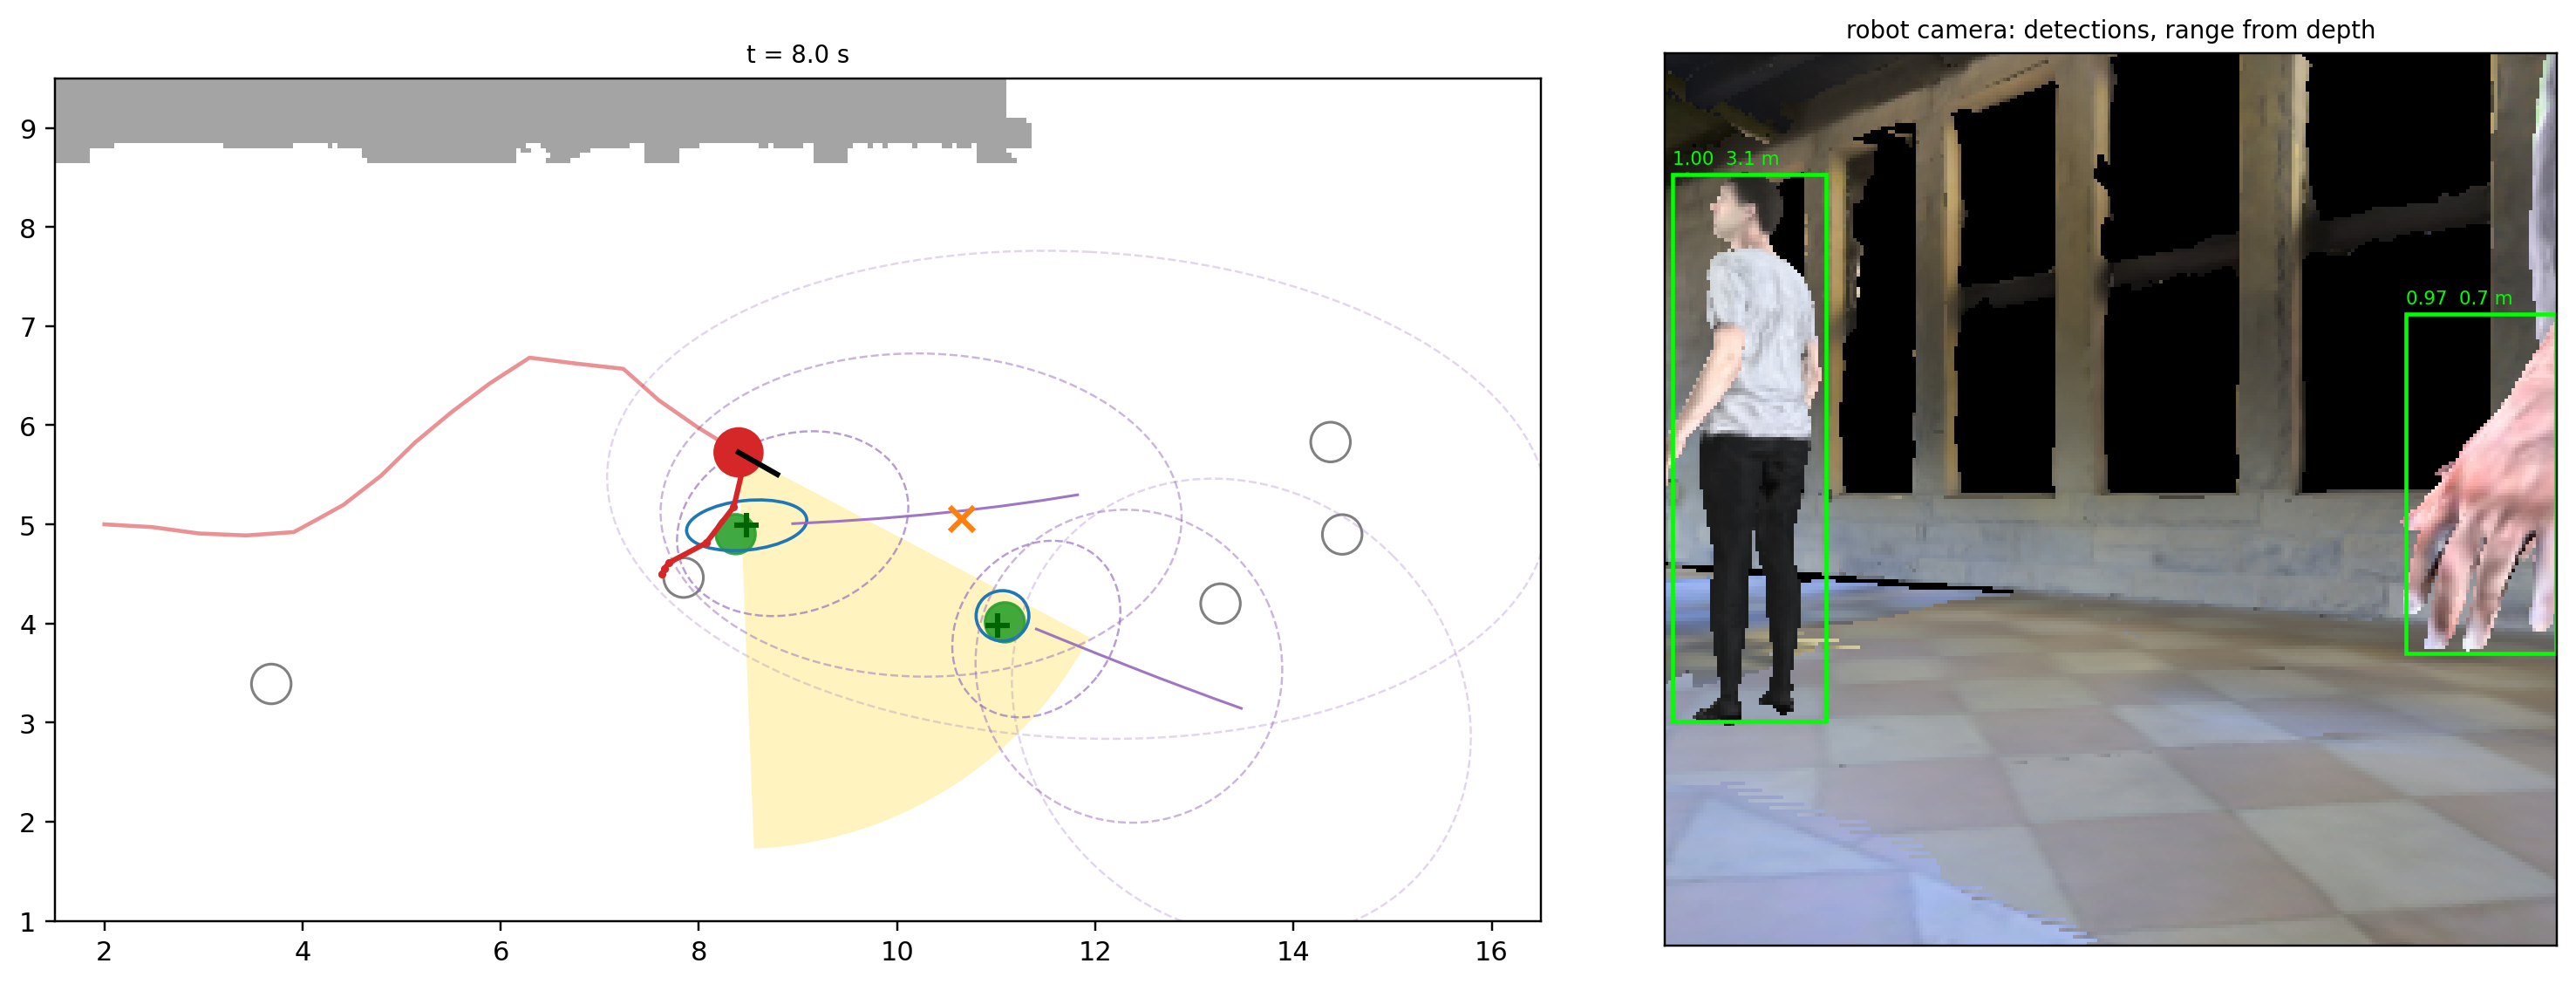
\includegraphics[width=0.74\textwidth]{fig_socnav.png}
\caption{SocNavBench Zara episode with RGB-D perception. Left: true pedestrians (green: detected), PMB tracks (blue), predictions (purple), the camera cone and the robot's plan. Right: the rendered robot view with detections (score, depth range).}
\label{fig:socnav}
\end{figure*}

\section{Results}

\subsection{Risk-aware gaze beats passive and heuristic gaze}
On 1,800 paired replay episodes (Table~\ref{tab:replay}) risk-aware gaze beats the fixed camera, scanning, look-at-nearest and the TTC heuristic ($p_\text{Holm} \le 0.003$), with 40\% fewer collisions with never-seen pedestrians than the fixed camera. It pays for them with more collisions with tracked pedestrians (757 vs.\ 534): looking around is looking away. The gaze oracle is only 4 points ahead, so pointing this camera better has little left to give; the 360$^\circ$ camera is 21 points ahead, so coverage is the real ceiling.

\begin{table}[t]
\centering
\caption{Replayed crowds, 1,800 paired episodes. Success excluding spawn collisions, collisions with never-seen and with tracked pedestrians, $p_\text{Holm}$ vs.\ ours.}
\label{tab:replay}
\footnotesize
\setlength{\tabcolsep}{4pt}
\begin{tabular}{lcccc}
\toprule
Gaze & Success & Never-seen & Tracked & $p_\text{Holm}$ \\
\midrule
Risk-aware (ours) & \textbf{0.643} & 964 & 757 & -- \\
Decoupled         & 0.644 & 880 & 832 & 0.55 \\
Information gain  & 0.629 & 1011 & 714 & 0.54 \\
Fixed             & 0.601 & 1605 & 534 & 0.003 \\
Look at nearest   & 0.599 & 1811 & 448 & 0.002 \\
TTC heuristic     & 0.584 & 1908 & 456 & $<$0.001 \\
Scan              & 0.577 & 1603 & 948 & $<$0.001 \\
\midrule
Gaze oracle       & 0.686 & 523 & 844 & \\
360$^\circ$ camera & 0.858 & 39 & 448 & \\
\bottomrule
\end{tabular}
\end{table}

\subsection{The objective matters, joint optimization does not}
Information gain ties the risk-aware objective (272:246, $p{=}0.27$), and so does the decoupled planner (263:265). What carries the gain is pointing the camera at uncertainty that threatens the path, not solving gaze and motion in one problem; the decoupled version is cheaper and equally good. In the ablations (Holm over eight), only the tracker and the tracked-pedestrian gaze term are individually necessary: a Kalman tracker instead of the PMB costs 5.5 points ($p_\text{Holm}{=}0.001$), dropping the tracked term 3.5 ($p_\text{Holm}{=}0.03$), dropping the unseen-pedestrian term 3.2 (borderline, $p_\text{Holm}{=}0.07$); the unseen constraint, existence weighting, stale-track pruning and the propagated state covariance show no measurable effect.

\subsection{Where it helps: dense crowds}
Splitting the episodes by the number of pedestrians near the straight-line path (Table~\ref{tab:density}), the benefit over the fixed camera is absent on sparse paths, 5 points at medium density and 7.5 in dense crowds, where risk-aware gaze also leads information gain (0.441 vs.\ 0.390), the only place in the replays where the two objectives separate. This split was made after the pre-registered analysis and is descriptive.

\begin{table}[t]
\centering
\caption{Success by crowd density (thirds by pedestrians near the path).}
\label{tab:density}
\footnotesize
\setlength{\tabcolsep}{3.5pt}
\begin{tabular}{lcccccc}
\toprule
Crowd & $n$ & Ours & Info.\ gain & Fixed & 360$^\circ$ & Ours vs.\ fixed \\
\midrule
Sparse & 690 & 0.790 & 0.796 & 0.780 & 0.938 & 84\,:\,77 ($p{=}0.64$) \\
Medium & 613 & 0.643 & 0.635 & 0.591 & 0.869 & 129\,:\,97 ($p{=}0.04$) \\
Dense  & 497 & 0.441 & 0.390 & 0.366 & 0.732 & 113\,:\,76 ($p{=}0.009$) \\
\bottomrule
\end{tabular}
\end{table}

\subsection{With real perception}
On SocNavBench's 30 curated episodes with ten fresh seeds (300 paired runs, Table~\ref{tab:socnav}), the three best replay alternatives were run against ours with the full vision pipeline. Risk-aware gaze gains 9 points over the fixed camera; the confidence interval excludes zero and the uncorrected test passes ($p{=}0.019$), but the Holm-corrected test narrowly misses ($p_\text{Holm}{=}0.056$). The leads over information gain and the decoupled planner are small, as in the replays. Replacing the simulated camera by the detector did not lower any method's success, so at 4\,m perception noise is not the bottleneck. The planner solves in about 90\,ms in replay and 400\,ms with vision (CPU, including the detector).

\begin{table}[t]
\centering
\caption{SocNavBench with RGB-D vision, 300 paired runs; difference to ours with 95\% cluster-bootstrap CI; one-sided episode-level permutation test, Holm-corrected.}
\label{tab:socnav}
\footnotesize
\begin{tabular}{lccc}
\toprule
Gaze & Success & Ours $-$ other (pts) & $p_\text{Holm}$ \\
\midrule
Risk-aware (ours) & \textbf{0.657} & -- & -- \\
Decoupled         & 0.633 & $+2.3$ $[-6.0, +10.3]$ & 0.29 \\
Information gain  & 0.603 & $+5.3$ $[-1.3, +12.3]$ & 0.17 \\
Fixed             & 0.567 & $+9.0$ $[+1.3, +16.7]$ & 0.056 \\
\bottomrule
\end{tabular}
\end{table}

\subsection{How good is the model of unseen pedestrians?}
We checked the Poisson part of the tracker against ground truth on 240 replay episodes. It ranks risk well, beating the static prior in log-likelihood for the next 1--3 steps, but it is biased low: it expects 0.74 of the untracked pedestrians in the scene and 0.65 of those within 4\,m outside the view, and the probability it assigns to an undetected pedestrian in a collision disk is about half the observed frequency around the planner's 2\% risk level. The constraint of (f) therefore binds at roughly 4\% rather than 2\%. On held-out episodes whose prior was fitted on earlier data of the same density the model is unbiased (ratio 1.10) and its detection probability matches the measured one (0.728 vs.\ 0.720 assumed), so the parameters are right; the bias comes from a density shift between the halves of each recording (1.1--2.3$\times$ more pedestrians in the second), which the single scene-wide multiplier only partly absorbs. Two remedies tried on calibration data only: a weak prior on the multiplier recovers a fifth of the gap (0.65 $\to$ 0.72) at no cost; a gaze term rewarding information about the density (the Gamma posterior's variance reduction) changes nothing. Restoring the intended 2\% risk ($\delta_u{=}0.01$) gives $+1.6$ points on the tuning seed, consistently but not significantly ($p{=}0.31$), and is not adopted.

\subsection{What did not help}
On the tuning seed, each tested and left out: a hybrid risk-plus-entropy objective, a time-to-contact term, path-swept relevance, calibrating the perception cost by detection history, pan-effort and horizon sweeps, a camera running at twice the control rate, predicting out-of-view tracks with the network instead of constant velocity, propagating track uncertainty through the predictor's sensitivity, and a slower robot (which hurt every method, since replayed pedestrians walk into it).

\section{Limitations}
\emph{Non-reactive crowd.} Replayed pedestrians ignore the robot, which penalizes exactly the caution the unseen-pedestrian terms add. \emph{Localization.} The robot pose is ground truth plus noise in both settings. \emph{Sensing.} In replay the camera is simulated; in SocNavBench detections are real but cut at 4\,m although the detector sees to 9\,m. \emph{Ceiling.} With this field of view, 21 of the 36 points to perfect perception are coverage that no gaze policy recovers. \emph{Statistics.} Two of three SocNavBench comparisons are underpowered at 300 runs; a 9-point effect needs about 500.

\section{Next Steps}
% TODO: assign owners; the names below are placeholders to be confirmed
\textbf{Paper (James Zhu).} A full-length RA-L manuscript from the extended abstract: related work on active perception, information-theoretic sensor control and perception-aware planning; the density analysis and the unseen-model calibration as the explanatory sections; a Fisher--Rao measurement of how much task-relevant information each gaze policy gathers per step, from the existing logs.

\textbf{Perception (Ahmed Ahmed, William Chan Santos).} Visual odometry in SocNavBench instead of ground-truth pose; detections beyond 4\,m with the measured range-dependent recall; a clutter model in the tracker so a detection sets $r_j<1$. Then a hardware test with a pan camera on the lab platform.

\textbf{Evaluation.} A reactive crowd (social-force pedestrians who avoid the robot), which changes what caution is worth; more SocNavBench seeds for the fixed-camera comparison; a realistic 87$^\circ$ camera.

\textbf{Guidance (Pinhas Ben-Tzvi).} Algorithm development and experiment design.

\bibliographystyle{IEEEtran}
\bibliography{ref}

\end{document}
